\documentclass{article}
\usepackage[utf8]{inputenc}

\title{Robustness and Sensitivity Analysis}
\author{Zhiyuan Chen}
\date{January 2018}

\usepackage{natbib}
\usepackage{graphicx}

\begin{document}

\maketitle

\section{Parameterization of the Productivity Evolution Process}
In Table \ref{robT1}, I present the coefficient estimates for the capital stock under different specifications for the productivity evolution process. Overall the estimates are close to each other. In the dataset, the value of capital stock ranges from 5.704 to 10.524, implying that the difference in productivity caused by the estimates of capital's coefficient is negligible. 


\begin{table}[h]
    \caption{Estimates of $\beta_{k}$ for different specifications}
    \label{robT1}
    \centering
    \begin{tabular}{cccc}
\hline\hline 
    Model &  linear & 2nd order & 3rd order \\
    \hline
     $\hat{\beta}_k$ & -0.0313\sym{**} & -0.0308\sym{**}&-0.0299\sym{**}  \\
                     &(-25.31)         &(-25.71)        &(-25.82) \\
   \hline
    \end{tabular}
\end{table}

Figure \ref{robfig1} shows that the distributions of productivity for specifications with higher ordered terms are more concentrated than the productivity estimates obtained from a linear specification. Note that for the linear specification, the constant term is not identified. On average, the productivity estimates with 3rd ordered term is the lowest.

Figure \ref{robfig2} shows that the slope of the productivity evolution equation has quite different patterns for different specifications. For the linear case, the slope is less than one and common for different productivity levels. For the 3rd ordered specification, the slope is hump-shaped with respect to the productivity, with a maximum slightly above the linear case but strictly less than one. For the case with 2nd order polynomials of productivity, the slope is stricly increasing in productivity, with a maximum greater than 1.1. Because firms have no incentive to invest in R\&D when its value function is infinite, the specification of 2nd-order polynomials actually implies the most productivity firms will not participate in R\&D, which is inconsistent with the stylized facts that many super productive firms undertake R\&D activities. 

\begin{figure}[h]
\caption{Distribution of the Productivity for Different Specifications}
\centering
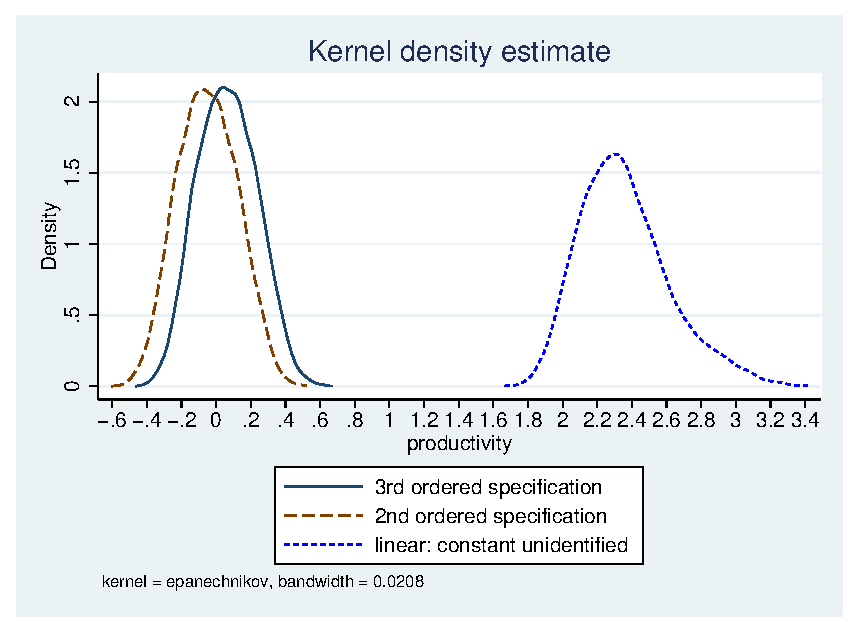
\includegraphics[width=0.8\textwidth]{RobustOmegaKdensity.eps}

\label{robfig1}
\end{figure}


\begin{figure}[h]
\caption{Distribution of the Slope for Different Specifications}
\centering
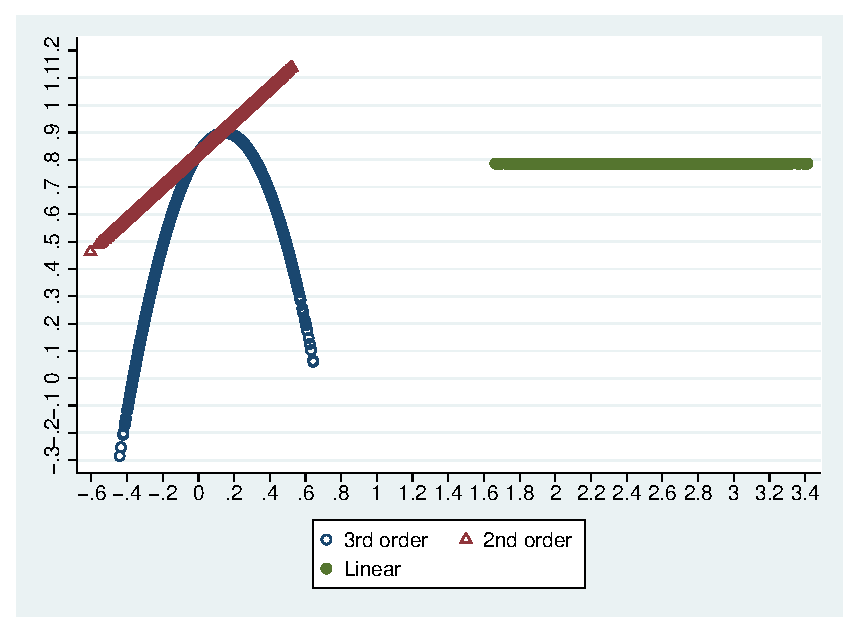
\includegraphics[width=0.8\textwidth]{RobustOmegaSlope.eps}

\label{robfig2}
\end{figure}




\end{document}
